%%%%%%%%%%%%%%%%%%%%%%%%%5
%% abtex2-modelo-trabalho-academico.tex, v<VERSION> laurocesar
%% Copyright 2012-<COPYRIGHT_YEAR> by abnTeX2 group at http://www.abntex.net.br/ 
%%
%% This work may be distributed and/or modified under the
%% conditions of the LaTeX Project Public License, either version 1.3
%% of this license or (at your option) any later version.
%% The latest version of this license is in
%%   http://www.latex-project.org/lppl.txt
%% and version 1.3 or later is part of all distributions of LaTeX
%% version 2005/12/01 or later.
%%
%% This work has the LPPL maintenance status `maintained'.
%% 
%% The Current Maintainer of this work is the abnTeX2 team, led
%% by Lauro César Araujo. Further information are available on 
%% http://www.abntex.net.br/
%%
%% This work consists of the files abntex2-modelo-trabalho-academico.tex,
%% abntex2-modelo-include-comandos and abntex2-modelo-references.bib
%%

% ------------------------------------------------------------------------
% ------------------------------------------------------------------------
% abnTeX2: Modelo de Trabalho Academico (tese de doutorado, dissertacao de
% mestrado e trabalhos monograficos em geral) em conformidade com 
% ABNT NBR 14724:2011: Informacao e documentacao - Trabalhos academicos -
% Apresentacao
% ------------------------------------------------------------------------
% ------------------------------------------------------------------------

\documentclass[
	% -- opções da classe memoir --
	12pt,				% tamanho da fonte
%  openright,			% capítulos começam em pág ímpar (insere página vazia caso preciso)
	twoside,			% para impressão em recto e verso. Oposto a oneside
	a4paper,			% tamanho do papel. 
	% -- opções da classe abntex2 --
	%chapter=TITLE,		% títulos de capítulos convertidos em letras maiúsculas
	%section=TITLE,		% títulos de seções convertidos em letras maiúsculas
	%subsection=TITLE,	% títulos de subseções convertidos em letras maiúsculas
	%subsubsection=TITLE,% títulos de subsubseções convertidos em letras maiúsculas
	% -- opções do pacote babel --
	english,			% idioma adicional para hifenização
	french,				% idioma adicional para hifenização
	spanish,			% idioma adicional para hifenização
	brazil				% o último idioma é o principal do documento
	]{abntex2}

% ---
% Pacotes básicos 
% ---
\usepackage{lmodern}			% Usa a fonte Latin Modern			
\usepackage[T1]{fontenc}		% Selecao de codigos de fonte.
\usepackage[utf8]{inputenc}		% Codificacao do documento (conversão automática dos acentos)
\usepackage{lastpage}			% Usado pela Ficha catalográfica
\usepackage{indentfirst}		% Indenta o primeiro parágrafo de cada seção.
\usepackage{color}				% Controle das cores
\usepackage{graphicx}			% Inclusão de gráficos
\usepackage{microtype} 			% para melhorias de justificação
% ---
		
% ---
% Pacotes adicionais, usados apenas no âmbito do Modelo Canônico do abnteX2
% ---
\usepackage{lipsum}				% para geração de dummy text
% ---

% ---
% Pacotes de citações
% ---
\usepackage[brazilian,hyperpageref]{backref}	 % Paginas com as citações na bibl
\usepackage[alf]{abntex2cite}	% Citações padrão ABNT

% --- 
% CONFIGURAÇÕES DE PACOTES
% --- 

% ---
% Configurações do pacote backref
% Usado sem a opção hyperpageref de backref
\renewcommand{\backrefpagesname}{Citado na(s) página(s):~}
% Texto padrão antes do número das páginas
\renewcommand{\backref}{}
% Define os textos da citação
\renewcommand*{\backrefalt}[4]{
	\ifcase #1 %
		Nenhuma citação no texto.%
	\or
		Citado na página #2.%
	\else
		Citado #1 vezes nas páginas #2.%
	\fi}%
% ---

% ---
% Informações de dados para CAPA e FOLHA DE ROSTO
% ---
\titulo{Características inerentes a medidas de centralidade e uso de algoritmos
de aprendizado de máquina para classificação de \textit{bridging nodes}}
\autor{Nome do autor}
\data{2018}
\local{Uberlândia}
\orientador{Prof.~Dr.~Anderson Rodrigues dos Santos}
\coorientador{}
\instituicao{%
  Universidade Federal de Uberlândia
  \par
  Programa de Pós-Graduação em Ciência da Computação
}
\tipotrabalho{Dissertação}

% O preambulo deve conter o tipo do trabalho, o objetivo (propósito), 
% o nome da instituição e a área de concentração.
% Esse texto irá compor a Folha de Rosto e Folha de Aprovação.
\preambulo{
% Propósito gerado automaticamente.
Dissertação apresentada ao Programa de Pós-Graduação em Ciência da Computação da Universidade Federal de Uberlândia, como requisito parcial para obtenção do grau de Mestrado em Ciência da Computação.
\newline\textbf{Área de concentração}: Computação.
\newline\textbf{Linha de pesquisa}: Inteligência Artificial.
}%% fim do preambulo




% ---
% Configurações de aparência do PDF final

% alterando o aspecto da cor azul
\definecolor{blue}{RGB}{41,5,195}

% informações do PDF
\makeatletter
\hypersetup{
     	%pagebackref=true,
		pdftitle={\@title}, 
		pdfauthor={\@author},
    	pdfsubject={\imprimirpreambulo},
	    pdfcreator={LaTeX with abnTeX2 and Limarka},
		pdfkeywords={abnt}{latex}{abntex}{abntex2}{trabalho acadêmico}{limarka}, 
		colorlinks=false,       		% false: boxed links; true: colored links
    	linkcolor=black,          	% color of internal links
    	citecolor=black,        		% color of links to bibliography
    	filecolor=black,      		% color of file links
		urlcolor=black,
		bookmarksdepth=4
}
\makeatother
% --- 

% ---
% Possibilita criação de Quadros e Lista de quadros.
% Ver https://github.com/abntex/abntex2/issues/176
%
\newcommand{\quadroname}{Quadro}
\newcommand{\listofquadrosname}{Lista de quadros}

\newfloat[chapter]{quadro}{loq}{\quadroname}
\newlistof{listofquadros}{loq}{\listofquadrosname}
\newlistentry{quadro}{loq}{0}

% configurações para atender às regras da ABNT
\setfloatadjustment{quadro}{\centering}
\counterwithout{quadro}{chapter}
\renewcommand{\cftquadroname}{\quadroname\space} 
\renewcommand*{\cftquadroaftersnum}{\hfill--\hfill}
% ---


% --- 
% Espaçamentos entre linhas e parágrafos 
% --- 

% O tamanho do parágrafo é dado por:
\setlength{\parindent}{1.3cm}

% Controle do espaçamento entre um parágrafo e outro:
\setlength{\parskip}{0.2cm}  % tente também \onelineskip

% ---
% compila o indice
% ---
\makeindex
% ---

%---
% CONFIGURAÇÕES EXTRA DO LIMARKA
%---

% Configura citações de pandoc para 4cm à esquerda (utiliza o ambiente quote)
\renewenvironment{quote}
  {\small\list{}{\rightmargin=0.1cm \leftmargin=4cm}%
   \item\relax}
  {\endlist}

% Para incluir páginas PDF (ficha catalografica e folha de aprovação)
\usepackage[dvipsnames]{xcolor} % http://tex.stackexchange.com/questions/124636/package-xcolor-error-undefined-colors-maroon-royal-blue-when-master-has-pdf
\usepackage{pdfpages}
\usepackage{longtable,ltcaption} % para as tabelas pandoc e quadros ABNT
%\usepackage{floatrow}
%\floatsetup[figure]{capposition=top}


% ---
% BUG: Imagens e tabelas apareciam no meio da página em branco 
% https://github.com/abntex/trabalho-academico-limarka/issues/1
% O código a seguir posta imagens ou tabelas em página em branco no topo, em vez do meio (comportamento padrão)
\makeatletter
\setlength{\@fptop}{5pt} % Set distance from top of page to first float
\makeatother
% ---

% ---
% Usado pelo limarka como hook para criação de novas listas.
% https://github.com/abntex/trabalho-academico-limarka/issues/16
%
\newcommand{\listasdousuario}{}


% ---
% CUSTOMIZAÇÕES DO USUÁRIO
% ---

\usepackage{latexcustomizacao} % importa customições do usuário.

%%
%% Esse modelo é responsável pela impressão dos seguintes elementos:
%% Capa, Folha de rosto e Ficha catalográfica.


% ----
% Início do documento
% ----
\begin{document}

% Seleciona o idioma do documento (conforme pacotes do babel)
%\selectlanguage{english}
\selectlanguage{brazil}

% Retira espaço extra obsoleto entre as frases.
\frenchspacing 

% ----------------------------------------------------------
% ELEMENTOS PRÉ-TEXTUAIS
% ----------------------------------------------------------
% \pretextual

% ---
% Capa
% ---
\imprimircapa
% ---

% ----------------------------------------------------------
% ELEMENTOS PRÉ-TEXTUAIS
% ----------------------------------------------------------
% \pretextual

% ---
% Folha de rosto: sempre será impressa
% ---
\imprimirfolhaderosto

% ---
% Sem ficha catalográfica
% ---
% ---


% ---
% ERRATA: Sem errata
% ---


% ---
% Sem Folha de aprovação
% ---
% ---

% ---
% Dedicatória
% ---
% ---
% Agradecimentos
% ---
% ---
% Epígrafe
% ---
% ---

% ---
% Resumo na língua vernácula (obrigatório)
% ---


% resumo em português
\setlength{\absparsep}{18pt} % ajusta o espaçamento dos parágrafos do resumo
\begin{resumo}

  As redes de interação proteína-proteína (PPI), com frequência, comportam
  números expressivos de nós (proteínas) e arestas (interações) na ordem
  dos milhares, possivelmente milhões. Os nós promissores em redes PPI de
  grande porte, passíveis a serem utilizados na produção de fármacos,
  podem ser identificadosatravés de métodos exatos como bridging
  centrality, no entanto, isto pode se tornar um problema computacional a
  ser superado devido à complexidade destas redes. Como alternativa, se
  sugere o uso de Inteligência Artificial, sendo o objetivo desta pesquisa
  analisar algoritmos de aprendizado de máquina (ML) aplicadas ao problema
  de determinação de bridging centrality em redes PPI, modeladas por meio
  de Rede Complexa, e identificar o algoritmo que ofereça resultados
  próximos ao gerado pelo algoritmo exato tido como referência, mas com
  esforço computacional menor. Foram selecionadas redes PPI de nove
  diferentes bactérias, sobre as quais foi gerado um conjunto de métricas
  estruturais usando o software Gephi. Em seguida, cada arquivo de PPI
  contendo as métricas geradas foi submetido à análise de 15 algoritmos
  selecionados para a ML, disponíveis no software WEKA. Os arquivos de
  métricas de predição foram submetidos ao melhor modelo preditivo
  identificado e, a seguir, os nós foram classificados em weak ou strong.
  Por fim, houve a avaliação do desempenho do classificador, utilizando-se
  o software R e o pacote ROCR, obtendo-se a curva ROC, o valor Area Under
  the Curve (AUC), a acurácia e o threshold correspondentes. Os melhores
  modelos de aprendizagem identificados foram gerados pelos algoritmos
  \textit{Bagging} e \textit{Random Forest}, e os piores foram gerados
  pelos algoritmos \textit{NaïveBayes} e \textit{OneR}. Em termos gerais,
  a acurácia média da predição foi de \(74,38\% \pm 5,84\%\), com limiar
  médio de \(96\%\), e AUC médio de \(65,09\% \pm 4,48\%\). Os nós
  preditos corretamente pelo classificador foram, em média, \(24,33\%\)
  sendo \(2,75\%\) verdadeiros positivos e \(21,58\%\) verdadeiros
  negativos. Por outro lado, \(75,66\%\) foram incorretamente
  classificados, sendo \(23,67\%\) falsos positivos e \(51,99\%\) falsos
  negativos. Comparando os \(2,75\%\) verdadeiros positivos com os
  identificados pelo algoritmo exato, obteve-se uma taxa de acerto médio
  de 77,16\% \pm 20,23\%. O resultado preditivo gerado pelo processo de ML
  aproximou-se do obtido pelo algoritmo exato, apresentando eficácia, no
  entanto, com considerável taxa de erro. Dessa forma, nossos resultados
  corroboram o conhecimento da literatura sobre uso de ML em redes
  complexas, ou seja, algoritmos de ML aplicados a medidas de centralidade
  complexas como a bridging centrality não são eficazes. O plugin
  implementado como um dos produtos deste trabalho para o software GEPHI,
  versão 0.9.1 ou superior, encontra disponível no site sourceforge.net,
  sob o nome de BridgingCentralityPlugin.

 \textbf{Palavras-chave}: PPI. Bridging Centrality. Aprendizado de Máquina. Redes Complexas
\end{resumo}


% ---
% Resumo em língua estrangeira (obrigatório)
% ---

% resumo em inglês
\begin{resumo}[Abstract]
 \begin{otherlanguage*}{english}
   Protein-protein interaction (PPI) networks often carry expressive
   numbers of proteins and interactions in the order of thousands, possibly
   millions. The promising nodes in large PPI networks, which can be used
   in drug production, can be identified through exact methods such as
   bridging centrality, however, this can become computationally expensive
   to be overcome due to the complexity of these networks. As an
   alternative, the use of machine learning is suggested. The objective of
   this study was analyzed machine learning algorithms (ML) applied to the
   problem of determining bridging centrality in PPI networks, modeled by
   Complex Network, and identify the algorithm which offers results closest
   to generated by the exact algorithm taken as a reference, but with less
   computational effort. PPI networks were selected from nine different
   bacteria, on which a set of structural metrics were generated using
   Gephi. Then, each PPI file containing the generated metrics was
   submitted to the analysis of 15 algorithms selected for ML available in
   the WEKA. The prediction metrics files were submitted to the best
   predictive model identified and then the nodes were classified as weak
   or strong. Finally, the performance of the classifier was evaluated
   using the R software and the ROCR package, obtaining the ROC curve, the
   area under ROC curve (AUC), the corresponding accuracy and threshold.
   The best learning models identified correspond to the algorithms Bagging
   and Random Forest and the worst were the NaiveBayes and OneR. In general
   terms, the mean prediction accuracy of the nodes of the PPIs was
   \(74.38\% \pm 5.84\%\), with a mean threshold of \(96\%\), and mean AUC
   of \(65.09\% \pm 4.48\%\). The nodes correctly predicted by the
   classifier were, on average, \(24.33\%\), with \(2.75\%\) true positive
   and \(21.58\%\) true negative. On the other hand, \(75.66\%\) were
   incorrectly classified, being \(23,67\%\) false positive and \(51.99\%\)
   false negative. Comparing the \(2.75\%\) true positive with those
   identified by the exact algorithm, an average hit rate of
   \(77.16\% \pm 20.23\%\) was obtained. The predictive result generated by
   the ML process approached that obtained by the exact algorithm,
   presenting efficacy, however, with a considerable error rate. Thus, our
   results corroborate the literature knowledge about the use of ML in
   complex networks, that is, ML algorithms applied to complex centrality
   measures such as bridging centrality are not effective. The plugin
   implemented as one of the products of this work for GEPHI software,
   version 0.9.1 or higher, is available on sourceforge.net under the name
   of BridgingCentralityPlugin.

   \vspace{\onelineskip}
 
   \noindent 
   \textbf{Keywords}: PPI. Bridging Centrality. Machine Learning. Complex Networks
 \end{otherlanguage*}
\end{resumo}


% ---

% ---
% Lista de ilustrações (opcional): não utilizando.
% ---


% ---
% Lista de quadros (opcional): não utilizando.
% ---

% Carrega listas definidas pelo usuário em `latexcustomizacao.sty`
\listasdousuario
% ---
% Lista de tabelas (opcional): não utilizando
% ---

% ---
% Lista de abreviaturas e siglas (opcional)
% ---
\begin{siglas}
  \item[ABNT] Associação Brasileira de Normas Técnicas
\end{siglas}
% ---

% ---
% Lista de símbolos (opcional): AUSENTE
% ---
% ---
% Sumário
% ---
\pdfbookmark[0]{\contentsname}{toc}
\tableofcontents*
\cleardoublepage
% ---


% ----------------------------------------------------------
% ELEMENTOS TEXTUAIS
% ----------------------------------------------------------
\textual
\pagestyle{simple}                  % #17 Cabeçalho apenas com 
\aliaspagestyle{chapter}{simple}    % a numeração das páginas


\chapter{Introdução}\label{introduuxe7uxe3o}

\section{Motivação}\label{motivauxe7uxe3o}

\section{Objetivos}\label{objetivos}

\subsection{Objetivo geral}\label{objetivo-geral}

Apresentação do objetivo geral.

\subsection{Objetivos específicos}\label{objetivos-especuxedficos}

\begin{itemize}
\tightlist
\item
  objetivo 1;
\item
  objetivo 2;
\item
  objetivo 3.
\end{itemize}

\chapter{Como utilizar recursos do
limarka}\label{como-utilizar-recursos-do-limarka}

\textbf{Consulte o wiki do projeto}:
https://github.com/abntex/limarka/wiki

Cada capítulo inicia automaticamente em página ímpar (em conformidade
com as Normas). Por isso que existem várias páginas em branco nesse
documento.

\section{Como citar e referenciar}\label{como-citar-e-referenciar}

O arquivo de referências é configurado em ``configuracao.pdf'',
utilize-o para gerenciar suas referências.

Veja um exemplo de citação direta e referenciação a seguir:

\begin{quote}
A `norma' 6023:2000 (2) é complicada e cheia de inconsistências. Jamais
será possível gerar um estilo bibtex totalmente consistente com a
`norma', até porque nem a `norma' é compatível com ela mesma. Um bom
estilo bibliográfico deve ter uma linha lógica para formatação de
referências. Assim, com alguns poucos exemplos, qualquer pessoa poderia
deduzir os casos omissos. Nesse sentido, a `norma' 6023 trafega pela
contra-mão. É quase impossível deduzir sua linha lógica. O problema mais
grave, no entanto, fica pela maneira de organizar nomes. A ABNT quebrou
o sobrenome em duas partes. Normalmente se fala apenas em ``\emph{last
name}'', mas agora temos o ``\emph{last last name}'' graças à ABNT.
\cite[p. 5]{abntex2cite}.
\end{quote}

Consulte o documento \citeonline{abntex2cite} para conhecer como
referenciar os conteúdos.

\section{Como inserir imagens}\label{como-inserir-imagens}

Por exemplo, a Figura \ref{passaro} mostra um pássaro que possui as
cores da bandeira do Brasil.

\begin{figure}[htbp]
\caption{Pássaro com as cores da bandeira do Brasil}\label{passaro}
\begin{center}
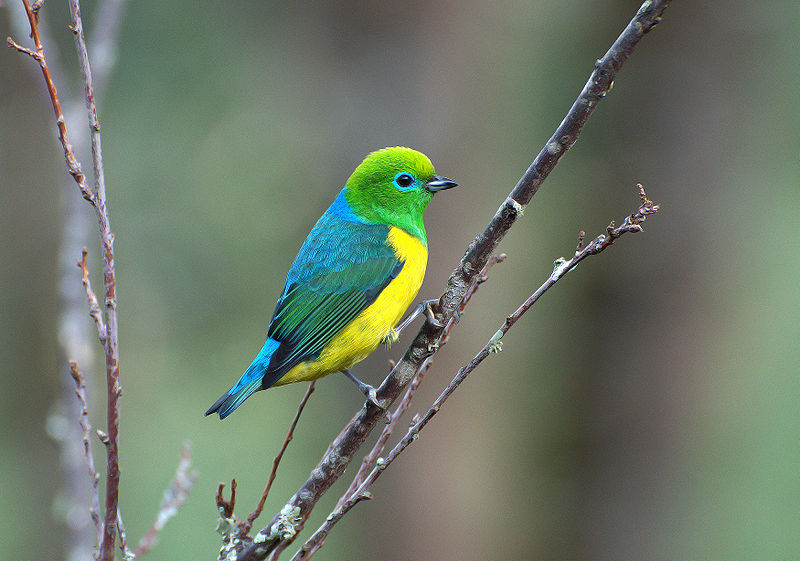
\includegraphics[width=0.40000\textwidth]{imagens/passaro.jpg}
\end{center}
\legend{Fonte: \citeonline{limarka}}
\end{figure}

As imagens são inseridas o mais próximo possível do texto que as
referenciam.

% ----------------------------------------------------------
% ELEMENTOS PÓS-TEXTUAIS
% ----------------------------------------------------------
\postextual
% ----------------------------------------------------------

% ----------------------------------------------------------
% Início dos ELEMENTOS PÓS-TEXTUAIS
% ----------------------------------------------------------
\postextual
% ----------------------------------------------------------

% ----------------------------------------------------------
% Referências bibliográficas
% ----------------------------------------------------------
\bibliography{xxx-referencias}
% ----------------------------------------------------------
% Apêndices
% ----------------------------------------------------------
% 
% ---
% Inicia os apêndices
% ---
\begin{apendicesenv}

% Imprime uma página indicando o início dos apêndices
\partapendices

\chapter{Primeiro apêndice}\label{primeiro-apuxeandice}

\lipsum[50]

\chapter{Segundo apêndice}\label{segundo-apuxeandice}

\lipsum[55-57]

\end{apendicesenv}

% ----------------------------------------------------------
% Anexos desativados: 
% Seção de anexos configurada como desativada
% ----------------------------------------------------------



\end{document}
